\documentclass[letterpaper, 12pt]{article}
\usepackage{amsmath}
\usepackage[margin=1in]{geometry}
\usepackage{adjustbox}
\usepackage{graphicx}
\usepackage[final]{pdfpages}
\usepackage{bm}
\usepackage{sectsty}
\usepackage{titlesec}
\usepackage{lipsum}
\usepackage{subcaption}
\usepackage{listings}
\usepackage{pgffor}
\usepackage{rotating}
\usepackage{xcolor}  
\usepackage{amsthm}
\usepackage{csvsimple}
\usepackage{enumitem}
\usepackage{amssymb} 
\usepackage{amsfonts}
\usepackage{tikz}
\usepackage{tikz-3dplot}
% \setlength{\tabcolsep}{0.5cm} 
\newcommand{\thickhat}[1]{\mathbf{\hat{\text{$#1$}}}}
\renewcommand{\lstlistingname}{Program}

\newtheoremstyle{custom}
  {3pt}
  {3pt}
  {\itshape}
  {} 
  {\bfseries}
  {. }  
  { }   
  {\thmname{#1} \thmnumber{#2} \thmnote{ #3}}

\theoremstyle{custom}


\newtheorem{definition}{Definition}
% \newtheorem{theorem}{Theorem}
\newtheorem*{theorem}{Theorem}
\sectionfont{\fontsize{12}{15}\selectfont}
\titleformat{\section}
{\normalfont\normalsize\bfseries}
{(\thesection)}{1em}{}

\title{Why Radians}
\author{Masaru Sawata}
\begin{document}
\maketitle
When I first learned about radians in high school, I wondered why angles are defined in such a strange way.  

At that time, I was taught that the arc length can be expressed as $r\theta$ (where $r$ is the radius and $\theta$ is the angle in radians).  
I didn't think this was very meaningful.  

However, when I learned about differentiation, I finally understood the purpose of introducing radians.  
What I will explain below may be something many people are already familiar with,  
but I believe it is a point that deserves more emphasis when we teach what radians are really for.

Let $x$ be a positive angle in degrees.  
(The same discussion applies if $x$ is negative.)

Now, consider the following arc and the two triangles shown below:
\begin{center}
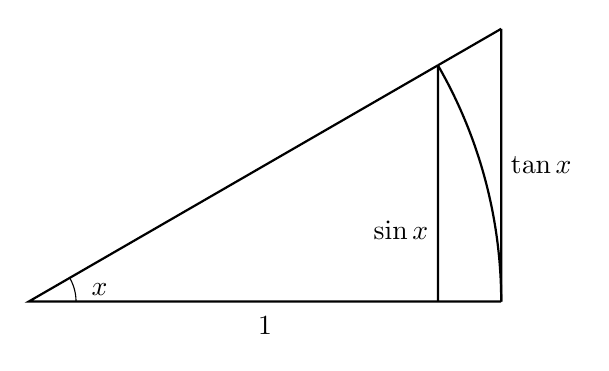
\begin{tikzpicture}[scale=6]
% Define angle
\def\angle{30}
\def\radius{1}

% Coordinates
\coordinate (O) at (0,0);
\coordinate (A) at (\radius,0);
\coordinate (B) at ({\radius*cos(\angle)}, {\radius*sin(\angle)});

% Triangle
\draw[thick] (A) -- (O) -- (B);

% Sine line
\draw[black, thick] (B) -- ({\radius*cos(\angle)},0);
\node[black, left] at ({\radius*cos(\angle)}, 0.15) {$\sin x$};

% Arc to represent angle x
\draw[black, thick] (A) arc (0:\angle:\radius);
% \node[red] at (0.8, 0.35) {arc length $\approx x$};

% Tangent line (dashed)
\draw[thick] (A) -- ({\radius}, {\radius*tan(\angle)});
\draw[thick] (B) -- ({\radius}, {\radius*tan(\angle)});
\node[right] at ({\radius}, {\radius*tan(\angle)/2}) {$\tan x$};

% Angle label
\draw[-] (0.1,0) arc (0:30:0.1);
\node at (0.15, 0.025) {$x$};
\node at (0.5, -0.05) {1};

% Point label
% \node[below right] at (B) {$(\cos x, \sin x)$};

\end{tikzpicture}
\end{center}

The arc length lies between the heights of the two triangles:
\begin{equation*}
  \sin x \leq 2 \pi \frac{x}{360} \leq \tan x
\end{equation*}
Dividing all sides by $\sin x$, we obtain:
\begin{equation*}
   \frac{180}{\pi} \leq \frac{x}{\sin x} \leq \frac{1}{\cos x}\frac{180}{\pi}
\end{equation*}
Taking the reciprocal:
\begin{equation*}
  \cos x \frac{\pi}{180} \leq \frac{\sin x}{x} \leq \frac{\pi}{180}
\end{equation*}
Therefore,
\begin{equation*}
  \lim_{x \rightarrow 0} \frac{\sin x}{x} = \frac{\pi}{180}
\end{equation*}

Now, consider the derivative of $\sin x$:
\begin{align*}
  \lim_{\Delta x \rightarrow 0} \frac{\sin (x+\Delta x) - \sin x}{\Delta x}
  &= \lim_{\Delta x \rightarrow 0} \frac{2 \cos \frac{2x+\Delta x}{2}\sin \frac{\Delta x}{2}}{\Delta x} \\
  &= \lim_{\Delta x \rightarrow 0} \cos \left( x+\frac{\Delta x}{2} \right) \frac{\sin \frac{\Delta x}{2}}{\frac{\Delta x}{2}} \\
  &= \frac{\pi}{180} \cos x
\end{align*}

As you can see, we would need to multiply by $\displaystyle \frac{\pi}{180}$ every time we take a derivative.  
This is quite cumbersome.

But if we use radians instead:
\begin{equation*}
  \lim_{x \rightarrow 0} \frac{\sin x}{x} = 1
\end{equation*}
So we no longer need to multiply by $\displaystyle \frac{\pi}{180}$.

This is a more convincing reason to introduce radians than simply saying they express arc length.
\end{document}